\usetikzlibrary{arrows.meta}
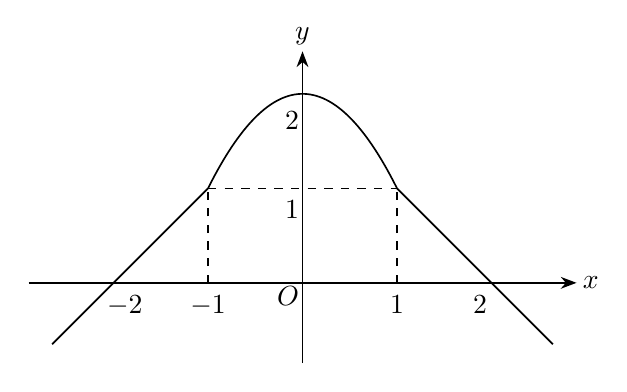
\begin{tikzpicture}[x=1.2cm,y=1.2cm,line width=.6pt,font=\normalsize,>=Stealth]
\draw[dashed] (-1,1)--(1,1);
\draw[dashed] (-1,0)--(-1,1);
\draw[dashed] (1,0)--(1,1);
\draw[->] (-2.9,0)--(2.9,0) node[right,inner sep=0pt,xshift=2pt] {$x$};
\draw[->] (0,-0.85)--(0,2.45) node[above,inner sep=0pt,yshift=2pt] {$y$};
\draw (-2.65,-0.65)--(-1,1);
\draw[domain=-1:1,samples=121] plot (\x,{2-\x*\x});
\draw (1,1)--(2.65,-0.65);
\node[below left,inner sep=1pt] at (0,0) {$O$};
\node[below,inner sep=1pt] at (-1.88,-0.10) {$-2$};
\node[below,inner sep=1pt] at (-1,-0.10) {$-1$};
\node[below,inner sep=1pt] at (1,-0.10) {$1$};
\node[below,inner sep=1pt] at (1.88,-0.10) {$2$};
\node[left,inner sep=1pt] at (0,0.78) {$1$};
\node[left,inner sep=1pt] at (0,1.72) {$2$};
\end{tikzpicture}
